% Options for packages loaded elsewhere
\PassOptionsToPackage{unicode}{hyperref}
\PassOptionsToPackage{hyphens}{url}
%
\documentclass[
]{article}
\title{inference\_regression\_lab}
\author{Brooke Wheeler}
\date{2/2/2022}

\usepackage{amsmath,amssymb}
\usepackage{lmodern}
\usepackage{iftex}
\ifPDFTeX
  \usepackage[T1]{fontenc}
  \usepackage[utf8]{inputenc}
  \usepackage{textcomp} % provide euro and other symbols
\else % if luatex or xetex
  \usepackage{unicode-math}
  \defaultfontfeatures{Scale=MatchLowercase}
  \defaultfontfeatures[\rmfamily]{Ligatures=TeX,Scale=1}
\fi
% Use upquote if available, for straight quotes in verbatim environments
\IfFileExists{upquote.sty}{\usepackage{upquote}}{}
\IfFileExists{microtype.sty}{% use microtype if available
  \usepackage[]{microtype}
  \UseMicrotypeSet[protrusion]{basicmath} % disable protrusion for tt fonts
}{}
\makeatletter
\@ifundefined{KOMAClassName}{% if non-KOMA class
  \IfFileExists{parskip.sty}{%
    \usepackage{parskip}
  }{% else
    \setlength{\parindent}{0pt}
    \setlength{\parskip}{6pt plus 2pt minus 1pt}}
}{% if KOMA class
  \KOMAoptions{parskip=half}}
\makeatother
\usepackage{xcolor}
\IfFileExists{xurl.sty}{\usepackage{xurl}}{} % add URL line breaks if available
\IfFileExists{bookmark.sty}{\usepackage{bookmark}}{\usepackage{hyperref}}
\hypersetup{
  pdftitle={inference\_regression\_lab},
  pdfauthor={Brooke Wheeler},
  hidelinks,
  pdfcreator={LaTeX via pandoc}}
\urlstyle{same} % disable monospaced font for URLs
\usepackage[margin=1in]{geometry}
\usepackage{color}
\usepackage{fancyvrb}
\newcommand{\VerbBar}{|}
\newcommand{\VERB}{\Verb[commandchars=\\\{\}]}
\DefineVerbatimEnvironment{Highlighting}{Verbatim}{commandchars=\\\{\}}
% Add ',fontsize=\small' for more characters per line
\usepackage{framed}
\definecolor{shadecolor}{RGB}{248,248,248}
\newenvironment{Shaded}{\begin{snugshade}}{\end{snugshade}}
\newcommand{\AlertTok}[1]{\textcolor[rgb]{0.94,0.16,0.16}{#1}}
\newcommand{\AnnotationTok}[1]{\textcolor[rgb]{0.56,0.35,0.01}{\textbf{\textit{#1}}}}
\newcommand{\AttributeTok}[1]{\textcolor[rgb]{0.77,0.63,0.00}{#1}}
\newcommand{\BaseNTok}[1]{\textcolor[rgb]{0.00,0.00,0.81}{#1}}
\newcommand{\BuiltInTok}[1]{#1}
\newcommand{\CharTok}[1]{\textcolor[rgb]{0.31,0.60,0.02}{#1}}
\newcommand{\CommentTok}[1]{\textcolor[rgb]{0.56,0.35,0.01}{\textit{#1}}}
\newcommand{\CommentVarTok}[1]{\textcolor[rgb]{0.56,0.35,0.01}{\textbf{\textit{#1}}}}
\newcommand{\ConstantTok}[1]{\textcolor[rgb]{0.00,0.00,0.00}{#1}}
\newcommand{\ControlFlowTok}[1]{\textcolor[rgb]{0.13,0.29,0.53}{\textbf{#1}}}
\newcommand{\DataTypeTok}[1]{\textcolor[rgb]{0.13,0.29,0.53}{#1}}
\newcommand{\DecValTok}[1]{\textcolor[rgb]{0.00,0.00,0.81}{#1}}
\newcommand{\DocumentationTok}[1]{\textcolor[rgb]{0.56,0.35,0.01}{\textbf{\textit{#1}}}}
\newcommand{\ErrorTok}[1]{\textcolor[rgb]{0.64,0.00,0.00}{\textbf{#1}}}
\newcommand{\ExtensionTok}[1]{#1}
\newcommand{\FloatTok}[1]{\textcolor[rgb]{0.00,0.00,0.81}{#1}}
\newcommand{\FunctionTok}[1]{\textcolor[rgb]{0.00,0.00,0.00}{#1}}
\newcommand{\ImportTok}[1]{#1}
\newcommand{\InformationTok}[1]{\textcolor[rgb]{0.56,0.35,0.01}{\textbf{\textit{#1}}}}
\newcommand{\KeywordTok}[1]{\textcolor[rgb]{0.13,0.29,0.53}{\textbf{#1}}}
\newcommand{\NormalTok}[1]{#1}
\newcommand{\OperatorTok}[1]{\textcolor[rgb]{0.81,0.36,0.00}{\textbf{#1}}}
\newcommand{\OtherTok}[1]{\textcolor[rgb]{0.56,0.35,0.01}{#1}}
\newcommand{\PreprocessorTok}[1]{\textcolor[rgb]{0.56,0.35,0.01}{\textit{#1}}}
\newcommand{\RegionMarkerTok}[1]{#1}
\newcommand{\SpecialCharTok}[1]{\textcolor[rgb]{0.00,0.00,0.00}{#1}}
\newcommand{\SpecialStringTok}[1]{\textcolor[rgb]{0.31,0.60,0.02}{#1}}
\newcommand{\StringTok}[1]{\textcolor[rgb]{0.31,0.60,0.02}{#1}}
\newcommand{\VariableTok}[1]{\textcolor[rgb]{0.00,0.00,0.00}{#1}}
\newcommand{\VerbatimStringTok}[1]{\textcolor[rgb]{0.31,0.60,0.02}{#1}}
\newcommand{\WarningTok}[1]{\textcolor[rgb]{0.56,0.35,0.01}{\textbf{\textit{#1}}}}
\usepackage{graphicx}
\makeatletter
\def\maxwidth{\ifdim\Gin@nat@width>\linewidth\linewidth\else\Gin@nat@width\fi}
\def\maxheight{\ifdim\Gin@nat@height>\textheight\textheight\else\Gin@nat@height\fi}
\makeatother
% Scale images if necessary, so that they will not overflow the page
% margins by default, and it is still possible to overwrite the defaults
% using explicit options in \includegraphics[width, height, ...]{}
\setkeys{Gin}{width=\maxwidth,height=\maxheight,keepaspectratio}
% Set default figure placement to htbp
\makeatletter
\def\fps@figure{htbp}
\makeatother
\setlength{\emergencystretch}{3em} % prevent overfull lines
\providecommand{\tightlist}{%
  \setlength{\itemsep}{0pt}\setlength{\parskip}{0pt}}
\setcounter{secnumdepth}{-\maxdimen} % remove section numbering
\ifLuaTeX
  \usepackage{selnolig}  % disable illegal ligatures
\fi

\begin{document}
\maketitle

\begin{Shaded}
\begin{Highlighting}[]
\FunctionTok{library}\NormalTok{(tidyverse)}
\end{Highlighting}
\end{Shaded}

\begin{verbatim}
## -- Attaching packages --------------------------------------- tidyverse 1.3.1 --
\end{verbatim}

\begin{verbatim}
## v ggplot2 3.3.5     v purrr   0.3.4
## v tibble  3.1.6     v dplyr   1.0.7
## v tidyr   1.1.4     v stringr 1.4.0
## v readr   2.1.1     v forcats 0.5.1
\end{verbatim}

\begin{verbatim}
## -- Conflicts ------------------------------------------ tidyverse_conflicts() --
## x dplyr::filter() masks stats::filter()
## x dplyr::lag()    masks stats::lag()
\end{verbatim}

\begin{Shaded}
\begin{Highlighting}[]
\NormalTok{women }\OtherTok{\textless{}{-}} \FunctionTok{read.csv}\NormalTok{(}\StringTok{"Mass\_Calorie\_Data{-}1.csv"}\NormalTok{, }\AttributeTok{header =} \ConstantTok{TRUE}\NormalTok{, }\AttributeTok{sep =} \StringTok{","}\NormalTok{)}
\FunctionTok{attach}\NormalTok{(women)}
\end{Highlighting}
\end{Shaded}

\hypertarget{we-want-to-fit-a-regression-model-that-predicts-calorie-rate-rate-in-calories-per-day-based-on-lean-body-mass-lbm-in-kg.}{%
\section{we want to fit a regression model that predicts Calorie Rate
(RATE) in calories per day based on Lean Body Mass (LBM) in
kg.}\label{we-want-to-fit-a-regression-model-that-predicts-calorie-rate-rate-in-calories-per-day-based-on-lean-body-mass-lbm-in-kg.}}

\hypertarget{start-by-fitting-the-regression-model.-find-the-values-of-the-least-squares-estimators-regression-coefficients-and-write-the-equation-of-the-lsr-line.}{%
\section{1. Start by fitting the regression model. Find the values of
the least-squares estimators (regression coefficients) and write the
equation of the LSR
line.}\label{start-by-fitting-the-regression-model.-find-the-values-of-the-least-squares-estimators-regression-coefficients-and-write-the-equation-of-the-lsr-line.}}

\begin{Shaded}
\begin{Highlighting}[]
\CommentTok{\# RATE = y}
\CommentTok{\# LBM = X}

\CommentTok{\# fitting a regression model}
\NormalTok{reg }\OtherTok{\textless{}{-}} \FunctionTok{lm}\NormalTok{(RATE }\SpecialCharTok{\textasciitilde{}}\NormalTok{ LBM)}

\NormalTok{reg}
\end{Highlighting}
\end{Shaded}

\begin{verbatim}
## 
## Call:
## lm(formula = RATE ~ LBM)
## 
## Coefficients:
## (Intercept)          LBM  
##      201.16        24.03
\end{verbatim}

\begin{Shaded}
\begin{Highlighting}[]
\CommentTok{\# least square estimators: {-}81.433}

\CommentTok{\# Least squares regression line: y= {-}81.433 + .159x}
\end{Highlighting}
\end{Shaded}

\hypertarget{plot-the-regression-line-in-a-color-other-than-black-with-the-data.-include-the-plot-here.}{%
\section{2. Plot the regression line (in a color other than black) with
the data. Include the plot
here.}\label{plot-the-regression-line-in-a-color-other-than-black-with-the-data.-include-the-plot-here.}}

\begin{Shaded}
\begin{Highlighting}[]
\NormalTok{reg}
\end{Highlighting}
\end{Shaded}

\begin{verbatim}
## 
## Call:
## lm(formula = RATE ~ LBM)
## 
## Coefficients:
## (Intercept)          LBM  
##      201.16        24.03
\end{verbatim}

\begin{Shaded}
\begin{Highlighting}[]
\FunctionTok{plot}\NormalTok{(LBM, RATE)}
\FunctionTok{abline}\NormalTok{(reg, }\AttributeTok{col =} \StringTok{"red"}\NormalTok{)}
\end{Highlighting}
\end{Shaded}

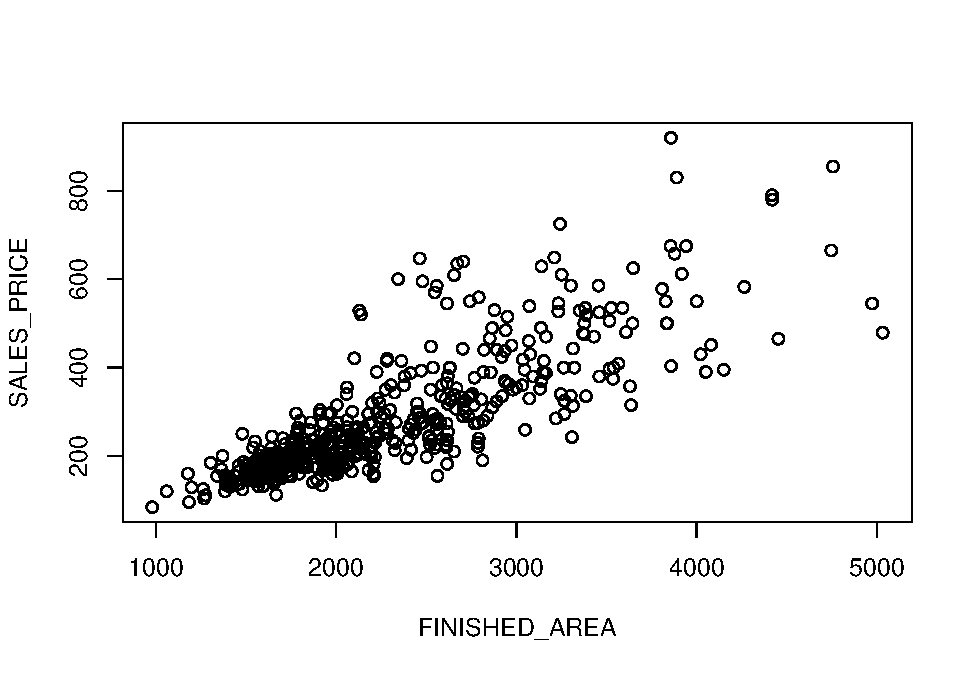
\includegraphics{inference_regression_lab_files/figure-latex/unnamed-chunk-3-1.pdf}
\# 3. Find a 98\% confidence interval for the slope, β\_1. Paste your
results below. Verify that your lower and upper limits match those from
the notes.

\begin{Shaded}
\begin{Highlighting}[]
\FunctionTok{confint}\NormalTok{(reg, }\AttributeTok{level =}\NormalTok{ .}\DecValTok{98}\NormalTok{)}
\end{Highlighting}
\end{Shaded}

\begin{verbatim}
##                    1 %     99 %
## (Intercept) -301.01781 703.3410
## LBM           12.49043  35.5617
\end{verbatim}

\begin{Shaded}
\begin{Highlighting}[]
\CommentTok{\# 98\% confidence interval for slop of B\_1 is 12.49043 to 35.5617}
\end{Highlighting}
\end{Shaded}

\hypertarget{what-does-the-98-confidence-interval-for-the-intercept-ux3b2_0-show-state-the-lower-and-upper-limits-and-discuss-what-they-mean-in-context.}{%
\section{4. What does the 98\% confidence interval for the intercept,
β\_0, show? State the lower and upper limits and discuss what they mean
in
context.}\label{what-does-the-98-confidence-interval-for-the-intercept-ux3b2_0-show-state-the-lower-and-upper-limits-and-discuss-what-they-mean-in-context.}}

\begin{Shaded}
\begin{Highlighting}[]
\FunctionTok{confint}\NormalTok{(reg, }\AttributeTok{level =}\NormalTok{ .}\DecValTok{98}\NormalTok{)}
\end{Highlighting}
\end{Shaded}

\begin{verbatim}
##                    1 %     99 %
## (Intercept) -301.01781 703.3410
## LBM           12.49043  35.5617
\end{verbatim}

\begin{Shaded}
\begin{Highlighting}[]
\CommentTok{\# the 98\% confidence interval for the intercept means that with 98\% confidence we estimate that the average (y) value of the intercept is between {-}301.01781 and 703.3410 meaning that when x is zero (if a women was to weigh 0 kg) then the rate of calories burned per day is between {-}301.01781 and 703.3410}
\end{Highlighting}
\end{Shaded}

\hypertarget{is-there-a-positive-association-between-lbm-and-calorie-rate-use-ux3b10.02.-state-the-hypotheses.-provide-the-value-of-sb_1-the-t-statistic-and-p-value.-do-they-match-those-found-in-the-notes-explain.}{%
\section{5. Is there a positive association between LBM and Calorie
Rate? Use α=0.02. State the hypotheses. Provide the value of s(b\_1),
the t statistic and p-value. Do they match those found in the notes?
Explain.}\label{is-there-a-positive-association-between-lbm-and-calorie-rate-use-ux3b10.02.-state-the-hypotheses.-provide-the-value-of-sb_1-the-t-statistic-and-p-value.-do-they-match-those-found-in-the-notes-explain.}}

\begin{Shaded}
\begin{Highlighting}[]
\CommentTok{\# null hyp:  slope = 0}
\CommentTok{\# alt. hyp:  slope \textgreater{}0}

\FunctionTok{summary}\NormalTok{(reg)}
\end{Highlighting}
\end{Shaded}

\begin{verbatim}
## 
## Call:
## lm(formula = RATE ~ LBM)
## 
## Residuals:
##    Min     1Q Median     3Q    Max 
## -95.87 -82.28  16.28  33.62 207.74 
## 
## Coefficients:
##             Estimate Std. Error t value Pr(>|t|)    
## (Intercept)  201.162    181.701   1.107 0.294169    
## LBM           24.026      4.174   5.756 0.000184 ***
## ---
## Signif. codes:  0 '***' 0.001 '**' 0.01 '*' 0.05 '.' 0.1 ' ' 1
## 
## Residual standard error: 95.08 on 10 degrees of freedom
## Multiple R-squared:  0.7682, Adjusted R-squared:  0.745 
## F-statistic: 33.13 on 1 and 10 DF,  p-value: 0.0001836
\end{verbatim}

\begin{Shaded}
\begin{Highlighting}[]
\CommentTok{\# s(b1)= 4.174}

\CommentTok{\# looking at the confidence interval for number 3 we found our 98\% confidence interval for slop of B\_1 is 12.49043 to 35.5617. Since zero is not in this interval we know we can reject the null hypothesis at level alpha=.02 and support that there is a positive association between LBM and calorie rate.}
\end{Highlighting}
\end{Shaded}

\hypertarget{note-the-value-of-residual-standard-error-shown-in-the-summary-of-the-regression-results.-what-does-this-correspond-to-hint-look-in-the-notes.-based-on-this-value-what-is-the-value-of-the-mse}{%
\section{6. Note the value of ``Residual standard error'' shown in the
summary of the regression results. What does this correspond to? (Hint:
Look in the notes.) Based on this value, what is the value of the
MSE?}\label{note-the-value-of-residual-standard-error-shown-in-the-summary-of-the-regression-results.-what-does-this-correspond-to-hint-look-in-the-notes.-based-on-this-value-what-is-the-value-of-the-mse}}

\begin{Shaded}
\begin{Highlighting}[]
\FunctionTok{summary}\NormalTok{(reg)}
\end{Highlighting}
\end{Shaded}

\begin{verbatim}
## 
## Call:
## lm(formula = RATE ~ LBM)
## 
## Residuals:
##    Min     1Q Median     3Q    Max 
## -95.87 -82.28  16.28  33.62 207.74 
## 
## Coefficients:
##             Estimate Std. Error t value Pr(>|t|)    
## (Intercept)  201.162    181.701   1.107 0.294169    
## LBM           24.026      4.174   5.756 0.000184 ***
## ---
## Signif. codes:  0 '***' 0.001 '**' 0.01 '*' 0.05 '.' 0.1 ' ' 1
## 
## Residual standard error: 95.08 on 10 degrees of freedom
## Multiple R-squared:  0.7682, Adjusted R-squared:  0.745 
## F-statistic: 33.13 on 1 and 10 DF,  p-value: 0.0001836
\end{verbatim}

\begin{Shaded}
\begin{Highlighting}[]
\CommentTok{\# residual standard error is 95.08}
\CommentTok{\# the residual standard error measures the average distance of residuals from the regression line. The residual standard eror corresponds to RMSE. This means that on average the residual is 95.08 away from the regression line. }

\CommentTok{\# MSE is 9040 calories per day. RMSE= 95.08}
\end{Highlighting}
\end{Shaded}


\end{document}
